\documentclass[12pt,fleqn]{article}\usepackage{../../common}
\begin{document}
Sıvı Dinamiğinde Sonlu Hacim Metotu - 1

Ağırlıklı Artıklar Metotu (Weighted Residual Method)

Önceki derste iyi koşullu bir sistemi elde etmeyi gördük, bu kötü koşullu (ill
conditioned) olmanın tersi tabii. Bu derste [1] AAM'yi kurmayı göreceğiz, ki bu
metot aslında kapsayıcı bir tarif, altında farklı hesap yöntemleri de
olabiliyor, AAM'nin kendisi hata kontrolünü nasıl yapacağımızı tarif ediyor.

Basit bir problemle başlayalım. Laplace formülü mesela, iki boyutu baz alalım,
ama birazdan göreceğimiz fikirler 1D ya da 3D için de geçerli. Problem bölgesi
(domain) $\Omega$ olsun onun sınırları $\Gamma$, 

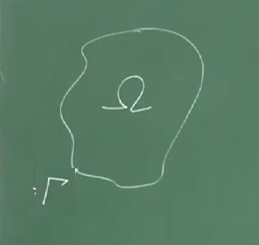
\includegraphics[width=15em]{compscieng_app45aerofem1_01.png}

İlgilendiğimiz alan (field) $T(x,y)$, bu reel değerli bir fonksiyon, ve
kurduğumuz sistem için bu fonksiyonun şu şartlara tabi olmasını istiyoruz,

$$
\nabla^2 T = 0 \quad \Omega \textrm{ üzerinde } 
$$

$$
\Gamma \textrm{ için } T = T_0
$$

Bu tur problemlere Drichlet problemleri deniyor.

Üstteki şartları yerine getiren bir $T(x,y)$ çözümü bulmak istiyoruz. O zaman
ilk akla gelen nedir? Diferansiyel denklemi alıyorum ve $\Omega$ içindeki tüm
noktalar için çözmeye uğraşıyorum. Fakat bu kolay değil. Ayrıca $\Omega$'daki
eşitlik $\Gamma$ sınırında geçerli değil, ikinci şart sebebiyle. Bu arada
matematiksel olarak çözüm nedir? $\Omega$'daki sonsuz tane nokta için geçerli
olan şeydir. Buna kesin çözüm (exact solution) deniyor. 

Fakat bu çözümü bulmak mümkün değilse, ya da yaklaşık bir çözüm de yeterli
oluyorsa o zaman yaklaşık yöntemler kullanabilirim.. $\nabla^2 T = 0 $ eşitliği
$\Omega$'daki her nokta için değil belli noktalar için, her $\Gamma$ noktasında
değil, belli noktalarda sınır şartı tatmin edilebilir diyebilirim.

``Belli noktalarda'' deyince iş bitmiyor, o seçilmiş noktalarda kesin çözüm mü
yapsam, yoksa o noktalarda da yaklaşık çözüm yapsam? Ya da tüm noktalarda
yaklaşık çözüm üzerinden bir hata hesaplayalım, tüm seçilmiş noktalarla 
hesaplanan ortalama bir hatanın sıfır olması için mi uğraşsam?

Şöyle bir yöntem deneyelim; elimizde / verili belli bir baz fonksiyon ``sınıfı''
olsun, bu fonksiyonlar Fourier bazı $\sin$, $\cos$ olabilir, ya da Chebisev
polinomları olabilir, bu ``test'' fonksiyonları $T_i(x,y)$ içinde olsun, ki
$i=1,2,...,N$, ve nihai $T$'yi

$$
T = T_0 + \sum _{i=1}^{N} c_i T_i(x,y)
$$

ile hesaplayabilirim, $c_i$'ler başta bilmediğim katsayı değerleri. Bilinen /
verili test fonksiyonları üzerinden doğru $c_i$'leri bulursam bu beni gerçek
fonksiyon $T$'ye yaklaştırır. Üstteki toplamda $T_0$ terimi özellikle o
şekilde formüle dahil edildi, $T_i$'lerin sınırda sıfır olmasını
ayarlayabilirsem, $T=T_0$ şartını o şekilde tatmin etmiş olurum.

$N$ sayısına dikkat, gerçek fonksiyonu aşağı yukarı temsil etmek istesem $N$'yi
az tutardım, birkaç tane temel fonksiyon birleşimi.. Ama $N$'i arttırarak, hatta
sonsuza yaklaştığımızda gerçek fonksiyona tıpatıp eşit olacağımızı
bekleyebilirdik, o zaman $N$ sayısı bir anlamda yaklaşıklamanın kalitesini
kontrol edecektir. $N$ arttıkça hata azalır, yaklaşıklama gerçeğe yaklaşır.
Bir ödünleşim (trade-off) durumu var muhakkak, çok büyük $N$ hesaplaması zor
olan bir sistem ortaya çıkartabilir, vs.

Bu bizi hata tanimina getiriyor. Onu artik (residual) uzerinden tanimlayacagiz,
artik $R$,

$$
R(c_i,x,y) = \nabla^2 T
$$

Bu kadar basit. Niye artığı direk $\nabla^2 T$'e eşitlemek yeterli? Çünkü ana
formüle bakarsak $\nabla^2 T$ ideal durumda sıfır olmalı değil mi?  Ama
yaklaşıklama mükemmel olmadığı için sıfırdan farklı (fakat umuyoruz ki ona
yakın) değerler döndürecektir, o zaman bu değeri alıp direk hata, artık olarak
kullanabiliriz.















[devam edecek]

Kaynaklar

[1] Mittal, {\em FEM for Fluid Dynamics, Lecture07 PartA, Method of Weighted Residuals, IIT Kanpur},
    \url{https://www.youtube.com/channel/UCWheqBdP45xBVp_Eqi1eltQ/videos}

\end{document}


